\documentclass{beamer}
\usetheme{Madrid} % theme
\usecolortheme{crane}
\title{Independent Project}
\subtitle{Stereo Speakers}
\author[Priyesh Pandey]{\textbf{Submitted to:Dr.GVV Sharma}\\  Priyesh Pandey\\EE16B1022} % auteur
\institute{\textbf {IIT Bhilai}}
\date{}
\titlegraphic{
\includegraphics[width=2cm]{logo.png}}
\begin{document}
\begin{frame}
  \titlepage
\end{frame}
\begin{frame}{}
  \begin{columns}
    \begin{column}{0.55\textwidth}
      
\begin{block}{\textbf{Objective}}
To make a commercial Stereo Speaker .
\end{block}
\begin{block}{\textbf{Components Used}}
\small
\begin{itemize}
  \item
    2 speakers
  \item
   4x22$\mu$F , 3x220$\mu$F and one 1000$\mu$F capacitors
  \item
   Voltage regulator
   \item
   Step-Down Transformer with 4 p-n Diodes
   \item
   2xLM386 IC
  \end{itemize}
\end{block}
    \end{column}
    \begin{column}{0.32\textwidth}
    \begin{center}
\begin{figure}[h]
\centering
\caption{\small Final Speakers as a product}
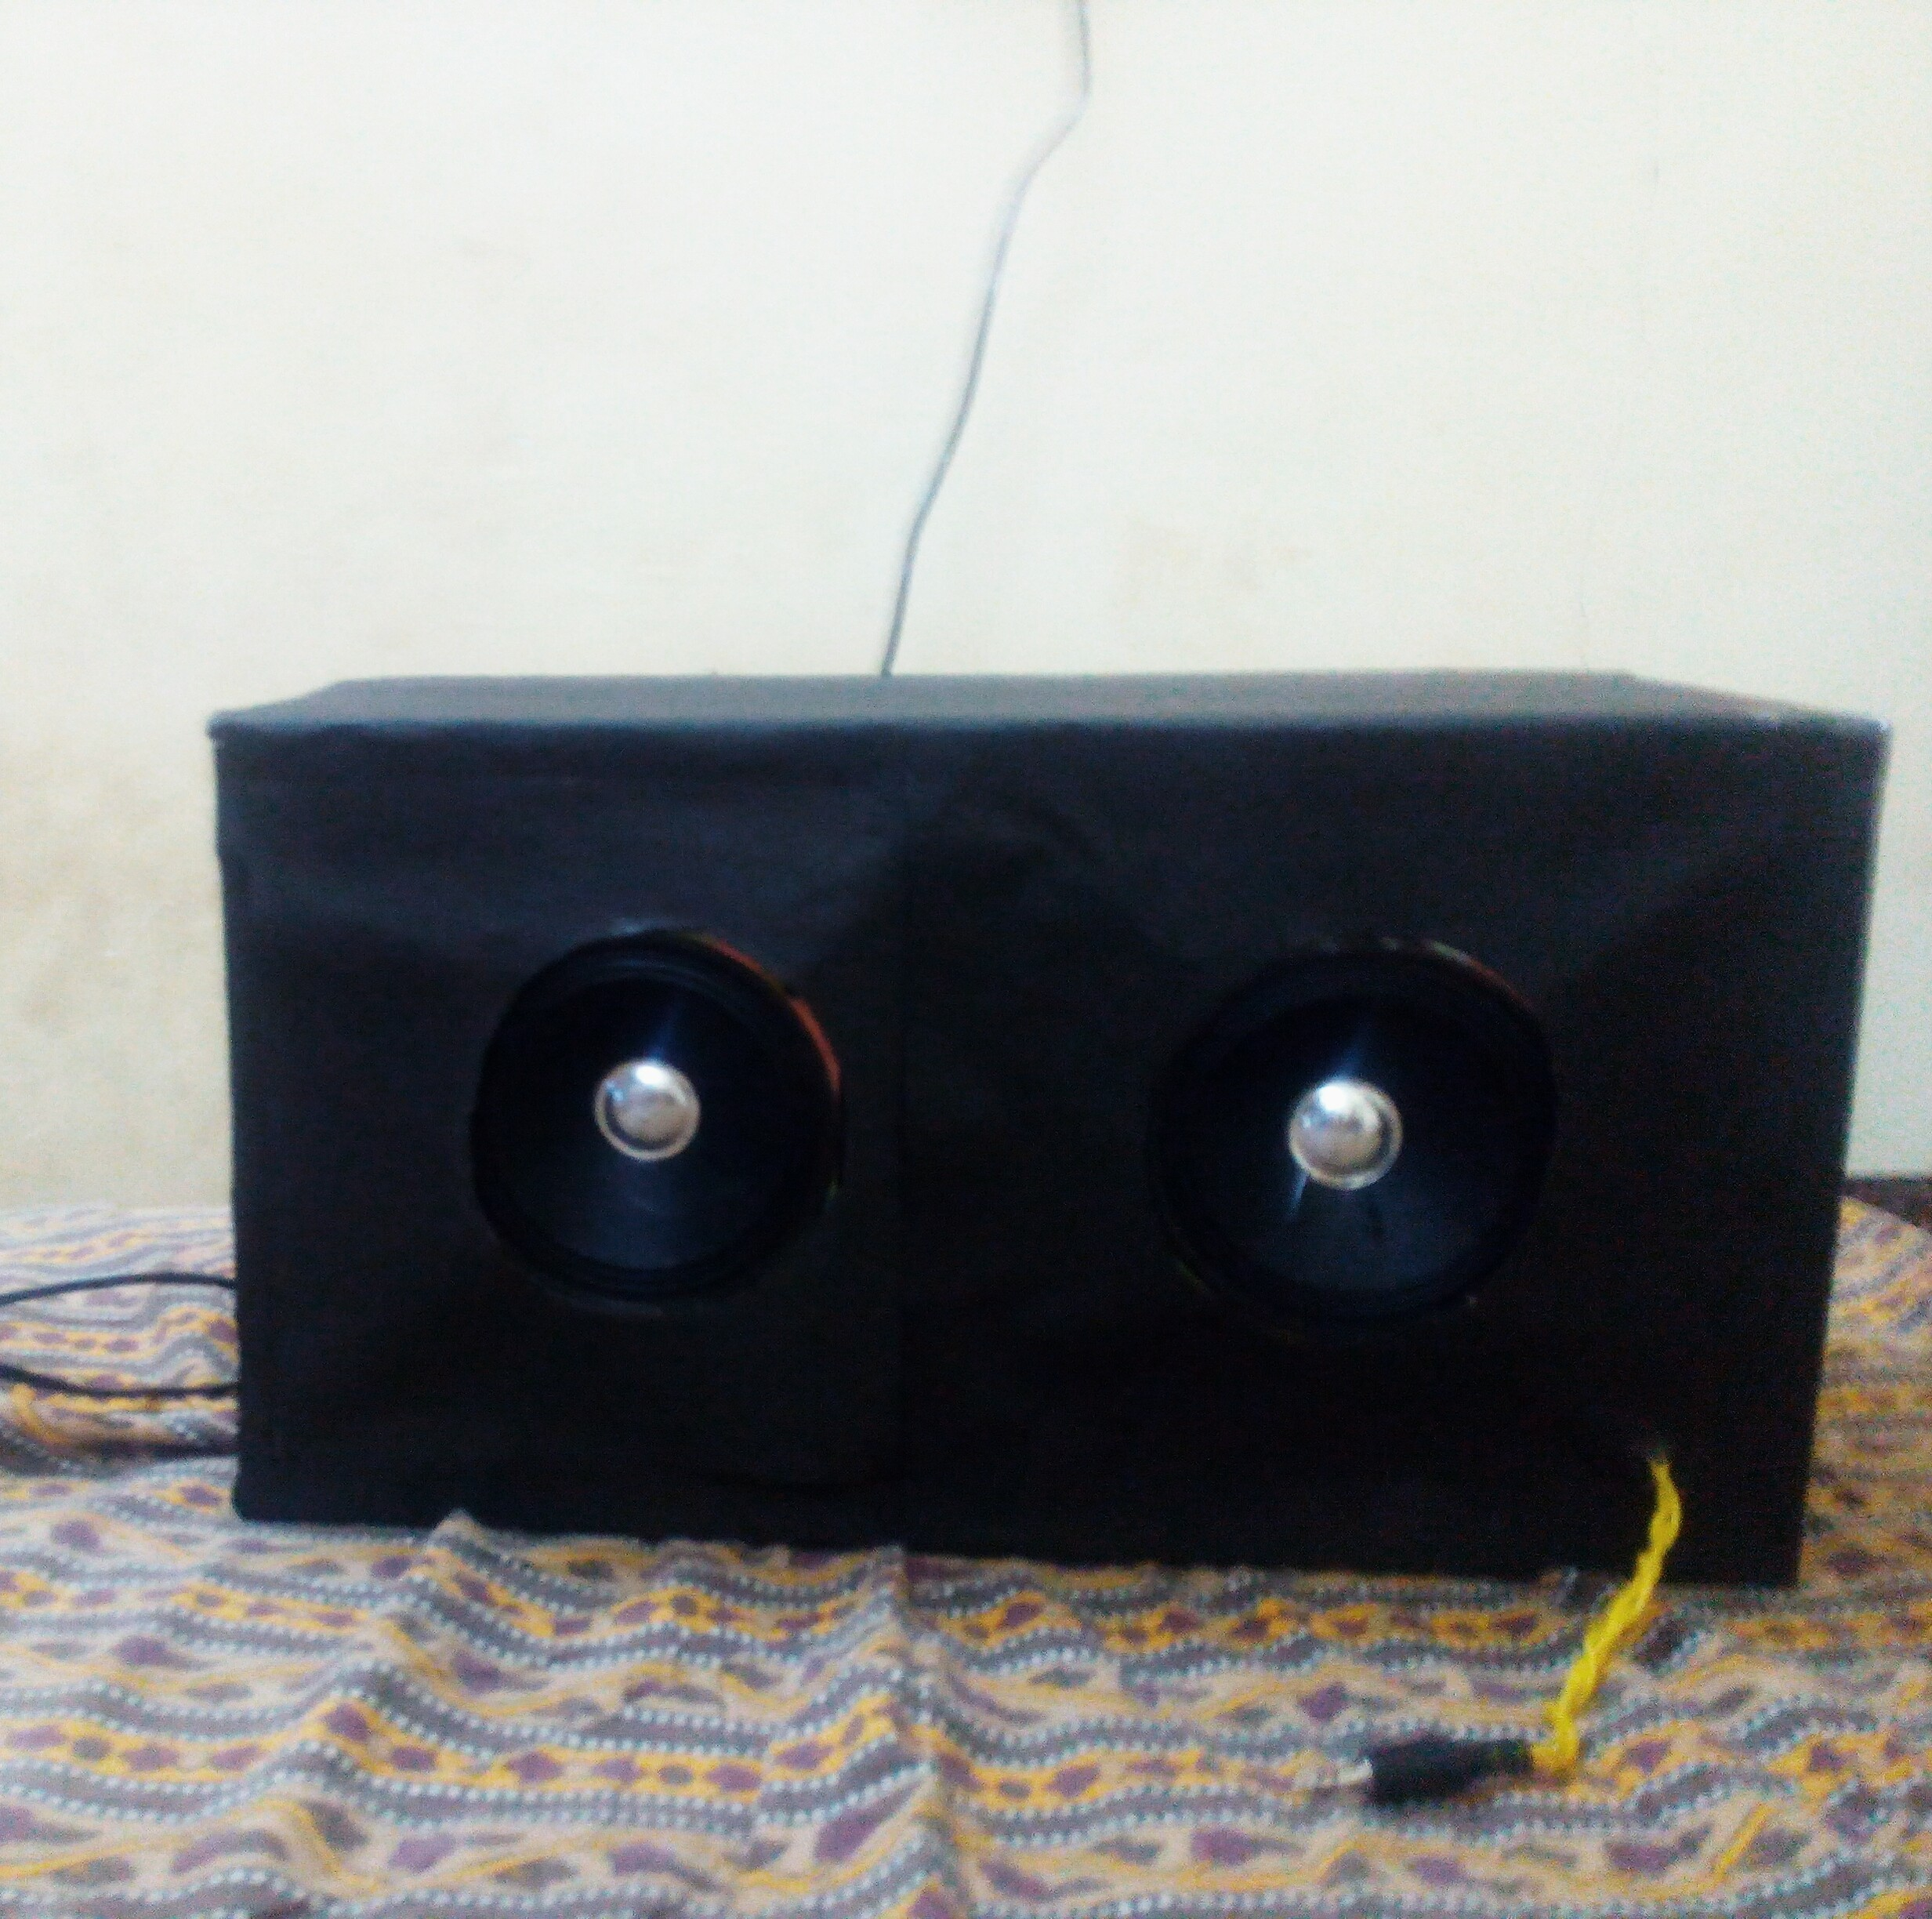
\includegraphics[width=\columnwidth]{12.jpg}
\end{figure}
\end{center}    
    \end{column}
\end{columns}
\end{frame}
\begin{frame}{Introduction}
  \begin{itemize}
  \item 
 We will use two speakers to create a stereo system.
  
  \item   
    The separate left and right sound channels of music  produces a stereo effect where slightly different sound is heard by the left and right ears, making it sound more "real".
  
  \item
    This project consists of two parts ,converting AC input to DC output for speakers and the audio amplification part. 
 
  \item
    For getting a DC output we have used the step-down transformer with diodes and capacitors also known as full wave rectifier
  \item
   For the audio amplification we have used LM386 IC's.
  \end{itemize}
\end{frame}

\begin{frame}{Working}{Full Wave rectifier}
  \begin{columns}
  \begin{column}{0.32\textwidth}
    \begin{center}
\begin{figure}[htb]
\centering
\caption{\small Wave output}
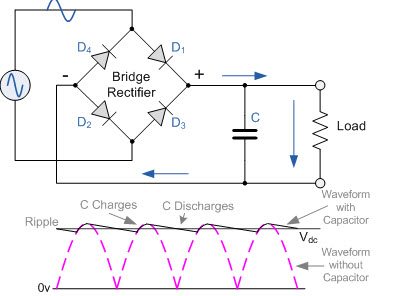
\includegraphics[width=\columnwidth]{5.jpg}
\end{figure}
\end{center}    
    \end{column}
    \begin{column}{0.55\textwidth}

\begin{itemize}
  \item
  In a full wave rectifier circuit we use two diodes, one for each half of the wave. Configuration results in each diode conducting in turn when its anode terminal is positive with respect to the transformer center point C produces an output during both half-cycles.
  \item
  IC 7809 acts a voltage regulator in this case and the capacitors are used to smoothen the output.
  
  \end{itemize}
  
    \end{column}
    
\end{columns}
\end{frame}

%\section*{Summary}

\begin{frame}{Working}{Audio amplifier}
  \begin{columns}
  \begin{column}{0.32\textwidth}
    \begin{center}
\begin{figure}[htb]
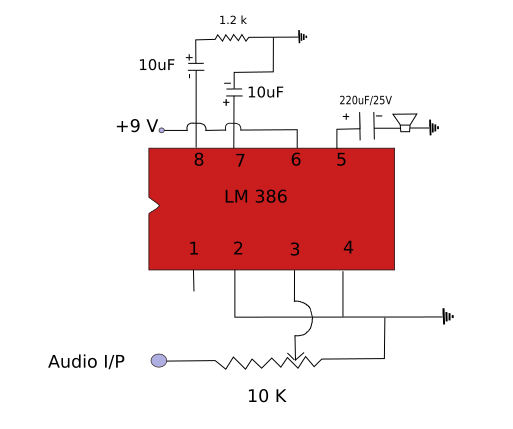
\includegraphics[scale=0.30]{7.png}
\caption{\small{LM 386 Circuit}}
\end{figure}
\end{center} 
 \end{column}
 \begin{column}{0.55\textwidth}
  \begin{itemize}
  \item
PIN 1 and 8: These are the gain control PINs, internally the gain is set to 20 but it can be increased up to 200 by using a capacitor between PIN 1 and 8.
\item
Pin 2 and 3: These are the input PINs for sound signals. Pin 2 is the negative input terminal to ground. Pin 3 is the positive input terminal, in which sound signal is fed to be amplified. In our circuit it is connected to the positive terminal of the audio jack with a  potentiometer. Potentiometer acts as volume control knob.
  \end{itemize}
  \end{column}
  \end{columns}
\end{frame}
\begin{frame}
\begin{itemize}
\item
Pin 4 and 6: These are the power supply Pins of IC, Pin 6 for is +Vcc and Pin 4 is Ground. The circuit can be powered with voltage between 5-12v.
\item
Pin 5: This is the output PIN, from which we get the amplified sound signal.
\item
The output signal has both AC and DC component, and DC component is undesirable and can’t be fed to Speaker. So to remove this DC component, a capacitor of 220uF has been used. 
Along with this capacitor, a filter circuit of Capacitor has been used at the output PIN 5.
\item
Pin 7: This is the bypass terminal. It can be left open or can be grounded using a capacitor for stability
\end{itemize}
\end{frame}
\begin{frame}{Implementation}
The input voltage is AC mains.So by use of step down transformer,we get a ac wave of 12v.Now by bridge rectifiers and capacitors the output is dc wave.Then we used IC 7809 which provides us with a 9V DC output.It also deals with fluctuations in the voltage,hence acts a a regulator.So from this we give power to our LM386 circuits.As we need to make two speakers functional so we use 2 LM386 to create stereo speakers.Now as the working of LM386 was stated,we use auio jack to provide input signal and get an amplified version of input signal as output signal on the speakers.   
    
\end{frame}
\end{document}
